% !TEX encoding = UTF-8 Unicode
\RequirePackage{fix-cm}
\documentclass[a4paper,10pt,UTF8]{paper}
%\documentclass[a4paper,10pt,UTF8]{ctexart}

\usepackage[english]{babel}
\usepackage{fancyhdr,array,lastpage,amsmath,mathtools,enumitem,graphicx,multirow,tocbibind,longtable,makecell,varwidth,titlesec,bm,booktabs,comment}
\usepackage{enumitem}
\usepackage{hyperref}
\hypersetup{hidelinks}
%\setCJKmainfont[BoldFont=Heiti SC Medium]{Songti SC Light}
%\setCJKsansfont{Heiti SC}

\usepackage[left=2.54cm,right=2.54cm,top=2.54cm,bottom=2.54cm]{geometry}
\usepackage[font=footnotesize,labelfont=bf]{caption}
\usepackage{tikz,flowchart}
\usepackage{ctex}
\usetikzlibrary{shapes,shapes.geometric,arrows,matrix,calc}
\usetikzlibrary{circuits.logic}
% \usetikzlibrary{circuits.logic.custom}
\usetikzlibrary{circuits.logic.IEC}
\usetikzlibrary{shadows}
\usepackage{listings}
\usepackage[Q=yes]{examplep}
\usepackage{fancyhdr}
\usepackage{alphalph}
\usepackage{indentfirst}

\newenvironment{sol}
  {\par\vspace{2mm}\noindent{\bf Solution}. }

\lstset{escapeinside=``, breaklines=true, frame=none, extendedchars=false, basicstyle=\ttfamily, showstringspaces=false}


\setlength{\parindent}{2em}
\setlength{\parskip}{1.5ex plus 0.5ex minus 0.2ex}
\linespread{1.1}

\bibliographystyle{plain}

\numberwithin{equation}{section}
\numberwithin{figure}{section}

\usepackage{karnaugh}
\usepackage{circuitikz}


\setcounter{secnumdepth}{3}
\setcounter{tocdepth}{3}

\title{华东师范大学计算机科学技术系上机实验报告}

\begin{document}
\pagestyle{fancy}
\chead{\small\color{gray}华东师范大学计算机科学技术系上机实验报告}
\lhead{}
\rhead{}
\makeatletter
\def\headrule{{\if@fancyplain\let\headrulewidth\plainheadrulewidth\fi%
\color{gray}\hrule\@height 0.2pt\@width\headwidth}
  \vspace{6mm}}
\makeatother

\newcommand{\HRule}{\rule{\linewidth}{1mm}}
\newcommand{\dai}{\textbf{Dais-CMX16$^+$}}

{\center {\huge \bfseries \LARGE{华东师范大学计算机科学技术系上机实验报告}} \\ [0.8cm]

\small{
  \begin{minipage}[t]{.32\linewidth}
    \textbf{课程名称:}计算机组成与结构实践\\
    \textbf{指导教师:}金健\\
    \textbf{上机实践名称:} 地址总线组成实验\\
    \textbf{实践编号:}实验 3
  \end{minipage}
  \begin{minipage}[t]{.32\linewidth}
    \textbf{年级:}17 级\\
    \textbf{姓名:}朱桐\\
    \textbf{学号:}10175102111\\
    \textbf{组号:}A
  \end{minipage} 
  \begin{minipage}[t]{.32\linewidth}
    \textbf{上机实践成绩:} \\
    \textbf{创新实践成绩:} \\
    \textbf{上机实践日期:}2019/09/29\\
    \textbf{上机实践时间:}2 学时\\
  \end{minipage}
}
\HRule \\[0.5cm]
}
\section{实验目的}

\begin{enumerate}
    \item 熟悉和了解地址总线的组成结构
    \item 掌握程序段和数据段的寻址规则及地址部件的运用技巧
    
\end{enumerate}

\section{实验设备}

\dai 一台

\section{实验内容}

向PC、AR和SP中分别存入一个数,并对PC中的数执行 PC+1

\section{实验原理}

地址总线的作用是传递地址信息,输出当前数据总线上发送信息的源地址或接收信息的目的 地址。如下图所示本系统设有内存与外设两条地址总线,通过 PC 计数器提供内存(程序存储器) 地址,并由地址寄存器 AR 传递内存(数据存储器)地址与外设地址。另外堆栈寄存器 SP 亦可 视为地址寄存器,它的堆顶指向数据与程序指针存取地址。

\subsection{11位程序地址}

\begin{figure}[h]
  \centering
  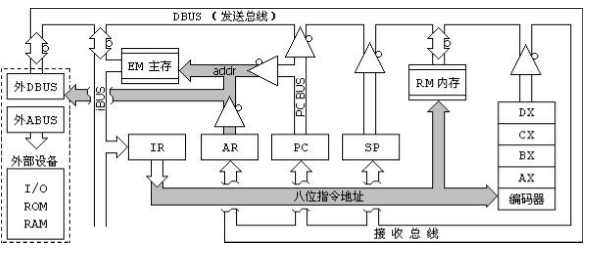
\includegraphics[width=0.7\textwidth]{1.PNG}
  \caption{地址总线组成通路}
  \label{fig:1}
\end{figure}

如图 \ref{fig:1} 所示,本系统从提高信息存取效率的角度设计主内存地址通路,按现代计算机体 系结构中最为典型的分段存取理念合成主存及外设地址总线 addr,在指令操作“时段” (取操作 码与取操作数) ,以当前程序指针 PC 为址,遇主存数据传递“时段”以当前数据指针 AR 为址。 addr 地址的合成通路见图 \ref{fig:1}。其寻址范围为 0~7FFh。

\subsection{16 位数据地址}

如图 \ref{fig:1} 所示,本系统数据指针由地址锁存器 AR 直接提供,当 LDAR=1 时,在 DRCK 下降沿把数据总线打入 AR。其寻址范围为 0~FFFFh,可达 64KB。

\begin{figure}[h]
  \centering
  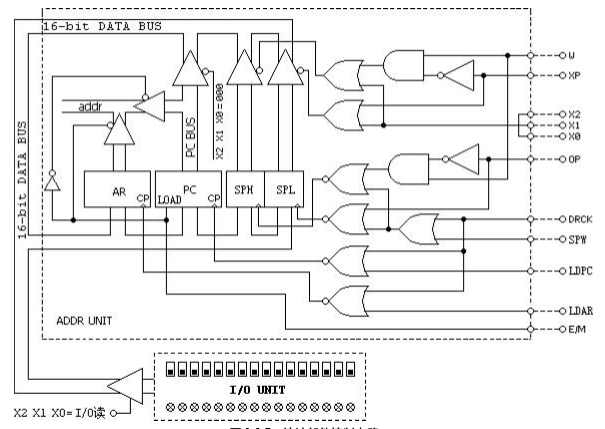
\includegraphics[width=0.9\textwidth]{2.PNG}
  \caption{地址部件控制电路}
  \label{fig:2}
\end{figure}

\subsection{程序计数器PC的操作}
\begin{figure}[h]
  \centering
  \begin{tabular}{|c|c|c|c|}
    \hline
    E/M & IP & DRCK & 功能 \\
    \hline
    0 & 0 & -- & PC保持 \\
    \hline
    0 & 1 & 脉冲 & PC=PC+1 \\
    \hline
    1 & 1 & 脉冲 & BUS->PC \\
    \hline
  \end{tabular}
  \caption{地址总线组成通路}
  \label{fig:3}
\end{figure}


程序计数器PC的操作如上表所示

\section{实验步骤}

\subsection{BUS 到 PC}

\begin{itemize}
  \item 设置 $E/M=0 IP=1, DRCK$ 脉冲
\end{itemize}


\subsection{BUS 到 SP}

\begin{itemize}
  \item 设置 $SPW=1, DRCK$ 脉冲
\end{itemize}


\subsection{BUS 到 AR}

\begin{itemize}
  \item 设置 $LDAR, DRCK$ 脉冲
\end{itemize}

\subsection{PC=PC+1}

\begin{itemize}
  \item 设置 $E/M=1 IP=1, DRCK$ 脉冲
\end{itemize}

\section{调试过程、结果与分析}

\subsection{实验结果}

实验结果如下列图片 \ref{fig:5},\ref{fig:6},\ref{fig:7},\ref{fig:8},\ref{fig:9} 所示


\begin{figure}[h]
  \centering
  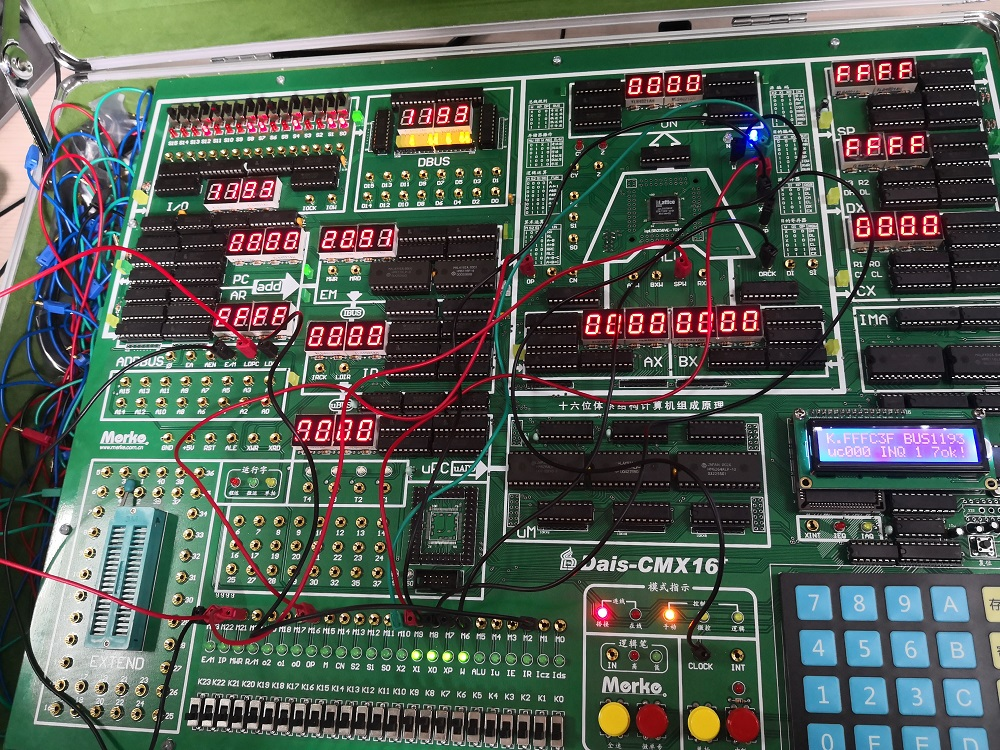
\includegraphics[width=0.9\textwidth]{io到总线.jpg}
  \caption{IO到总线}
  \label{fig:5}
\end{figure}

\begin{figure}[h]
  \centering
  \includegraphics[width=0.9\textwidth]{bus到pc.jpg}
  \caption{总线到PC}
  \label{fig:6}
\end{figure}

\begin{figure}[h]
  \centering
  \includegraphics[width=0.9\textwidth]{bus到sp.jpg}
  \caption{总线到AR}
  \label{fig:7}
\end{figure}

\begin{figure}[h]
  \centering
  \includegraphics[width=0.9\textwidth]{bus到sp.jpg}
  \caption{总线到SP}
  \label{fig:8}
\end{figure}

\begin{figure}[h]
  \centering
  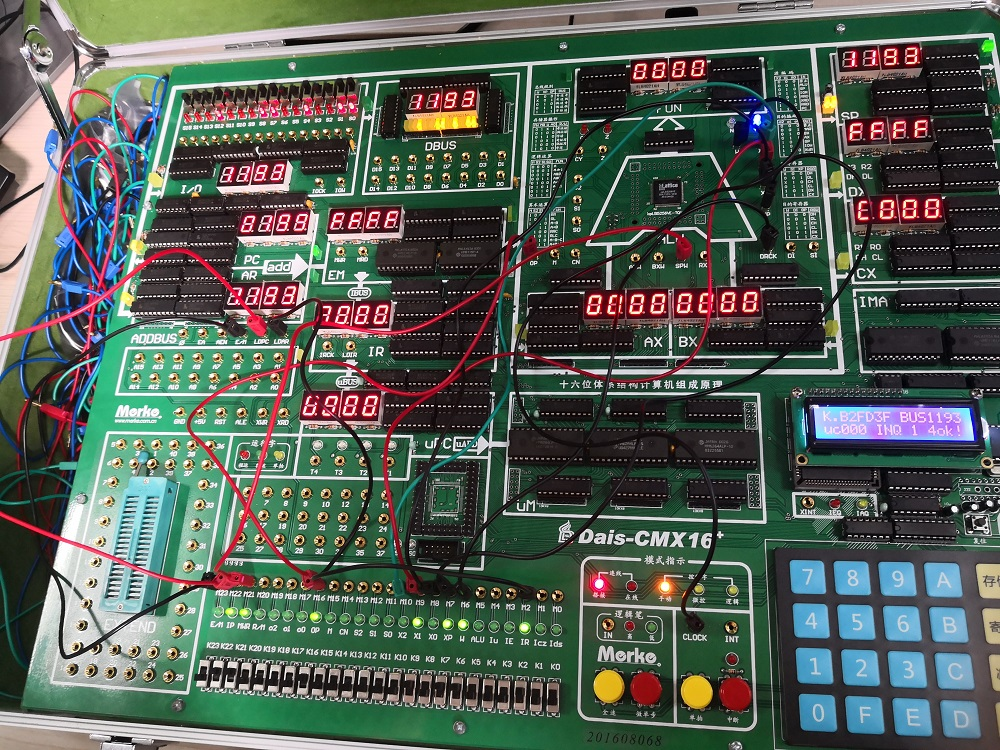
\includegraphics[width=0.9\textwidth]{pc+1.jpg}
  \caption{PC=PC+1}
  \label{fig:9}
\end{figure}


\subsection{调试过程与分析}

该次实验较为简单,没有调试过程。实验内容顺利完成。

\section{总结}

\begin{enumerate}
  \item 在开始之前最好首先了解每个开关的意义,帮助理解并且减少失误
  \item 开关最好插在下方对应表示的开关口中,剩余的按照表格填入。这样方便记忆每个插口的位置
  \item 每次开始之前先初始化
  \item 仔细阅读实验指导书
  \item 实验箱上每个模块的奇偶位输入都有对应的指示灯,方便指认电路是否连接错误
\end{enumerate}{}

\section{附件}

无

\end{document}
